\section{Standard ISO/IEC 9126}

\textit{ISO/IEC 9126} è uno standard internazionale che individua una serie
di normative per migliorare la qualità di prodotto.

\begin{figure}[h!]
	\centering
	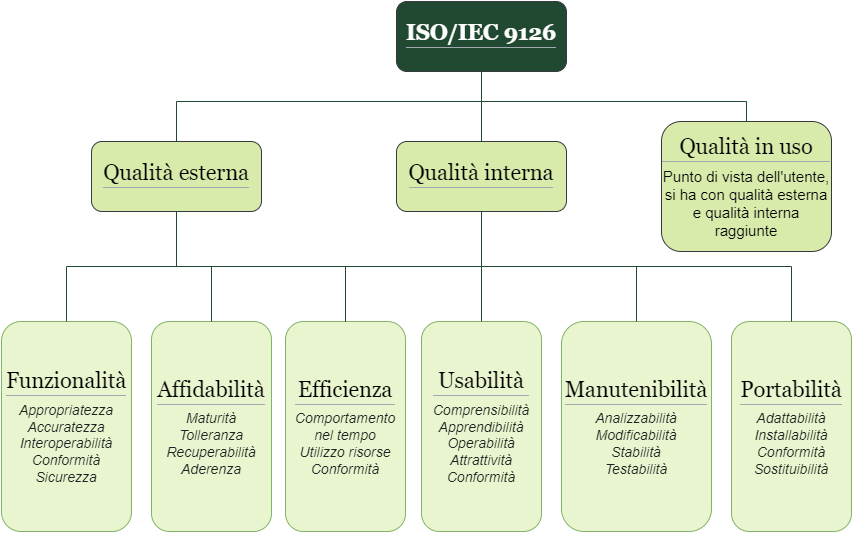
\includegraphics[scale=0.50]{../../assets/Norme_di_progetto/ISO9126.png}
	\caption{Rappresentazione del modello ISO/IEC 9126}
\end{figure}

\subsection{Modello di qualità}
Il modello di qualità descritto nello standard è caratterizzato da sei
caratteristiche generali:
\begin{enumerate}
	\item \textbf{Funzionalità}
	\begin{itemize}
		\item \textbf{Appropriatezza}: capacità del prodotto software di fornire un appropriato insieme
		di funzioni per specifici compiti ed obiettivi prefissati.
		\item \textbf{Accuratezza}: capacità del prodotto software di fornire i risultati 
		concordati o i precisi effetti richiesti.
		\item \textbf{Interoperabilità}: capacità del prodotto software di interagire ed operare con 
		uno o più sistemi.
		\item \textbf{Conformità}: capacità del prodotto software di aderire a standard, convenzioni e 
		regolamentazioni del settore operativo a cui vengono applicate.
		\item \textbf{Sicurezza}: capacità del prodotto software di proteggere informazioni e dati
		a persone o sistemi non autorizzati.
	\end{itemize}
	\item \textbf{Affidabilità}
	\begin{itemize}
		\item \textbf{Maturità}: capacità del prodotto software di evitare che si verifichino errori, 
		malfunzionamenti o siano prodotti risultati non corretti.
		\item \textbf{Tolleranza agli errori}: capacità del prodotto software di mantenere livelli predeterminati di prestazioni
		anche in presenza di malfunzionamenti o usi scorretti.
		\item \textbf{Recuperabilità}: capacità del prodotto di ripristinare il livello appropriato di prestazioni e di recupero 
		delle informazioni rilevanti, in seguito a un malfunzionamento.\\ Misura in particolare la quantità di tempo che impiega il
		prodotto software a tornare accessibile dopo un evento avverso.
		\item \textbf{Aderenza}: capacità del prodotto ad aderire a standard, regole e convenzioni inerenti all'affidabilità.
	\end{itemize}
	\item \textbf{Efficienza}
	\begin{itemize}
		\item \textbf{Comportamento nel tempo}: capacità di fornire adeguati tempi di risposta, elaborazione e velocità di attraversamento, 
		sotto condizioni determinate.
		\item \textbf{Utilizzo delle risorse}: capacità di utilizzo adeguato di quantità e tipo di risorse.
		\item \textbf{Conformità}: capacità del prodotto di aderire a standard e specifiche\\ sull'efficienza.
	\end{itemize}
	\item \textbf{Usabilità}
	\begin{itemize}
		\item \textbf{Comprensibilità}: facilità per l'utente di comprensione dei concetti del prodotto.
		\item \textbf{Apprendibilità}: riduzione dell'impegno richiesto all'utente per l'apprendimento dell'applicazione.
		\item \textbf{Operabilità}: capacità di mettere in condizione gli utenti di fare uso del prodotto software e controllarne l'uso.
		\item \textbf{Attrattività}: capacità del prodotto software di essere piacevole per l'utente che lo utilizza.
		\item \textbf{Conformità}: capacità del prodotto di aderire a standard e convenzioni relativi all'usabilità.
	\end{itemize}
	\item \textbf{Manutenibilità}
	\begin{itemize}
		\item \textbf{Analizzabilità}: facilità con la quale è possibile analizzare il codice per localizzare un errore.
		\item \textbf{Modificabilità}:capacità del prodotto software di permettere l'implementazione di una specificata modifica.
		\item \textbf{Stabilità}: capacità del prodotto software di evitare effetti inaspettati derivanti da modifiche errate.
		\item \textbf{Testabilità}: capacità del prodotto software di essere facilmente testato per validare le modifiche apportate.
	\end{itemize}
	\item \textbf{Portabilità}
	\begin{itemize}
		\item \textbf{Adattabilità}: capacità del prodotto software di essere adattato per differenti ambienti operativi.
		\item \textbf{Installabilità}: capacità del prodotto software di essere installato in uno specificato ambiente.
		\item \textbf{Conformità}: capacità del prodotto software di aderire a standard e convenzioni relative alla portabilità.
		\item \textbf{Sostituibilità}: capacità del prodotto software di essere utilizzato al posto di un altro software per svolgere 
		gli stessi compiti nello stesso ambiente.
	\end{itemize}
\end{enumerate}


\subsection{Technical Reports}
Nelle sezioni \textit{9126-2, 3} e \textit{4} dello standard vengono descritte
tre \textit{relazioni tecniche} per misurare le caratteristiche del modello di qualità.
\setlength\extrarowheight{5pt}

\begin{table}[h!]
    \centering
    \begin{tabular}{c|p{0.70\linewidth}}
    \rowcolor[RGB]{33, 73, 50}
    \multicolumn{1}{>{\centering\arraybackslash}c|}{\textcolor{white}{\textbf{Categoria}}} 
        & \multicolumn{1}{>{\centering\arraybackslash}c}{\textcolor{white}{\textbf{Descrizione}}} \\[4pt]
        \rowcolor[RGB]{216, 235, 171}
        \textbf{Qualità esterna}
        & Misura i comportamenti del software sulla base dei \textbf{test}: dall'operatività e 
		dall'osservazione durante la sua esecuzione. \\[4pt]
        \rowcolor[RGB]{233, 245, 206}
        \textbf{Qualità interna} 
        & Si applica alle parti di software \textbf{non eseguibili} (codice sorgente)
		durante le fasi di progettazione e codifica.
		Permette di prevedere la qualità esterna ed in uso, in quanto 
		gli attributi interni influiscono su quelli esterni ed in uso. \\[4pt]
        \rowcolor[RGB]{216, 235, 171}
        \textbf{Qualità in uso} 
        & Rappresenta il \textbf{punto di vista dell'utente} sul software \\[4pt]
    \end{tabular}
    \caption{Tipologie di qualità}
\end{table}

\subsubsection{Qualità in uso}
La qualità in uso permette di abilitare specificati utenti ad ottenere specificati obiettivi con:
\begin{itemize}
	\item \textbf{Efficacia}: la capacità del software di permettere agli utenti di raggiungere gli obiettivi specificati
	con accuratezza e completezza.
	\item \textbf{Produttività}: la capacità di permettere agli utenti di spendere una quantità di risorse
	appropriate in relazione all'efficacia ottenuta in uno specifico contesto d'uso.
	\item \textbf{Soddisfazione}: la capacità del prodotto software di soddisfare gli utenti.
	\item \textbf{Sicurezza}: la capacità del prodotto software di raggiungere accettabili livelli 
	di rischio di danni a: persone, software, apparecchiature e ambiente operativo d'uso.
\end{itemize}

\setlength\extrarowheight{0pt}